\documentclass{article}

\usepackage[preprint]{neurips_2019}

\usepackage[utf8]{inputenc} % allow utf-8 input
\usepackage[T1]{fontenc}    % use 8-bit T1 fonts
\usepackage{hyperref}       % hyperlinks
\usepackage{url}            % simple URL typesetting
\usepackage{booktabs}       % professional-quality tables
\usepackage{amsfonts}       % blackboard math symbols
\usepackage{nicefrac}       % compact symbols for 1/2, etc.
\usepackage{microtype}      % microtypography
\usepackage{amsmath}
\usepackage{subcaption}

\usepackage{pgfplots}
\pgfplotsset{compat=1.14}
\usepackage{tikz}
\usepackage{graphicx}
%\usepackage[square,numbers]{natbib}

\title{Hierarchical Deep Q-Network from Imperfect Demonstrations in Minecraft}

\author{%
Alexey Skrynnik\\
Artificial Intelligence Research Institute FRC CSC RAS\\
\texttt{skrynnik@isa.ru} \\
\And
Aleksey Staroverov\\
Moscow Institute of Physics and Technology\\
\texttt{alstar8@yandex.ru} \\
\And
Ermek Aitygulov\\
Moscow Institute of Physics and Technology\\
\texttt{aytygulov@phystech.edu} \\
\And
Kirill Aksenov\\
Higher School of Economics\\
\texttt{kaaksyonov@edu.hse.ru} \\
\And
Vasilii Davydov\\
Moscow Aviation Institute\\
\texttt{dexfrost89@gmail.com} \\
\And
Aleksandr I. Panov\\
Artificial Intelligence Research Institute FRC CSC RAS\\
Moscow Institute of Physics and Technology\\
\texttt{panov.ai@mipt.ru} \\
}

\begin{document}

    \maketitle

    \begin{abstract}
        We present Hierarchical Deep Q-Network (HDQfD) that won first place in the MineRL competition.
        The HDQfD works on imperfect demonstrations and utilizes the hierarchical structure of expert trajectories.
        We introduce the procedure of extracting an effective sequence of meta-actions and subgoals from the demonstration data.
        We present a structured task-dependent replay buffer and an adaptive prioritizing technique that allow the HDQfD agent to gradually erase poor-quality expert data from the buffer.
        In this paper, we present the details of the HDQfD algorithm and give the experimental results in the Minecraft domain.
    \end{abstract}


    \section{Introduction}\label{sec:introduction}
    Deep reinforcement learning (RL) has achieved compelling success on many complex sequential decision-making problems, especially in simple domains.
    In such examples as AlphaStar~\cite{vinyals2019alphastar}, AlphaZero~\cite{silver2017mastering},
    OpenAI Five human or superhuman performance was attained.
    However, RL algorithms usually require a huge amount of environment-samples required for training to reach good performance~\cite{kakade2003sample}.
    Learning from demonstration is a well-known alternative, but until now, this approach has not achieved any considerable success in complex non-single-task environments.
    This was largely due to the fact that obtaining high-quality expert demonstrations in a sufficient quantity in sample-limited, real-world domains is a separate non-trivial problem.

    Minecraft as a compelling domain for the development of reinforcement and imitation learning based methods was recently introduced by~\cite{guss2019minerl}.
    Minecraft presents unique challenges because it is a 3D, first-person, open-world game where the agent should gather resources and create structures and items to achieve a goal.
    Due to its popularity as a video game it turned out to be possible to collect a large number of expert trajectories in which individual subtasks are solved.
    This allowed the appealing MineRL competition to run.
    The organizers have released the largest-ever dataset of human demonstrations on a Minecraft domain.
    The primary goal of the competition is to foster the development of algorithms that can efficiently leverage human priors to drastically reduce the number of samples needed to solve complex, hierarchical, and sparse environments.

    The main difficulty in solving the MineRL problem was the imperfection of demonstrations and the presence of hierarchical relationships of subtasks.
    In this paper we present hierarchical Deep Q-Network from Demonstrations (HDQfD) that allowed us to win first place in the MineRL competition proposed by~\cite{guss2019minerl2}.
    The HDQfD works on imperfect demonstrations and utilize a hierarchical structure of expert trajectories extracting effective sequence of meta-actions and subgoals.
    Each subtask is solved by its own simple strategy, which extends the DQfD approach proposed by~\cite{gao2018reinforcement} and relies on a structured buffer and gradually decrease the ratio of poor-quality expert data.
    In this paper, we present the details of our algorithm and provide the results that allow the HDQfD agent to play Minecraft at the human level.


    \section{Background}\label{sec:background}

    One way to explore the domain with the use of expert data is to do behavioral cloning (BC).
    Pure supervised learning BC methods suffer from a distribution shift, because the agent greedily imitates the demonstrated actions, it can drift away from the demonstrated states due to error accumulation.
    Another way to use expert data in search for the exploration policy is to use conventional RL methods like PPO, DDDQN, etc.
    and guide exploration through enforcing occupancy measure matching between the learned policy and current demonstrations.

    The main approach is to use demonstration trajectories sampled from an expert policy to guide the learning procedure by either putting the demonstrations into a replay buffer or using them to pre-train the policy in a supervised manner.

    The organizers of the MineRL competition provided a few baselines.
    Standard DQfD presented by~\cite{hester2018deep} get the max score of 64 after 1000 episodes, the PPO gets the max of 55 after 800 episodes, the rainbow also gets the max of 55 after 800 episodes of training.

    Our best solution exploits the method of injecting expert data into the agent replay buffer.
    The DQfD, which our method is based on, is an advanced approach to reinforcement learning with additional expert demonstrations.
    The main idea of the DQfD is to use an algorithm called Deep Q-Network (DQN) and combine loss function $J(Q)$, with the main component $J_E(Q)$:
    \begin{equation}
        J(Q) = J_{DQ}(Q) + {\lambda_1}J_n(Q) + {\lambda_2}J_E(Q) + {\lambda_3}J_{L2}(Q).
        \label{eq:losses}
    \end{equation}
    The loss function $J_{DQ}(Q)$ is a standard TD-error:
    \begin{equation}
        J_{DQ}(Q) = \left( R(s,a) + \gamma Q(s_{t+1}, a^{\max}_{t+1}; \theta') - Q(s, a; \theta) \right)^2.\label{eq:td}
    \end{equation}
    The loss function $J_n(Q)$ is the so-called N-step return, which allows the agent to extend the utility of trajectories to several steps, which lead to a better strategy:
    \begin{equation}
        J_n(Q) = r_t + {\gamma}r_{t+1} + \dots + \gamma^{n-1}r_{t+n-1} + max_{a}\gamma^{n}Q(s_{t+n}, a).\label{eq:n-step}
    \end{equation}
    The main part $J_E(Q)$ is a margin loss function.
    It is responsible for copying expert behavior and gives a penalty to the agent for performing actions other than those of the experts:
    \begin{equation}
        J_E(Q) = \max_{a \in A}[Q(s, a) + l(a_E, a)] - Q(s, a_E).\label{eq:margin}
    \end{equation}
    Finally, $J_{L2}(Q)$ is L2 regularization added to prevent overfitting.

    The problem of suboptimal demonstrations is considered by~\cite{nair2018overcoming}, who attempted to develop an approach closely related to ours.
    The authors use the BC loss as a margin loss only for expert data.
    The key idea of the suggested approach is Q-Filter, which applies the BC loss only to the states where the critic determines that the action of the demonstrator is better than that of the actor.
    The use of expert demonstrations depends on the quality of the critic, which can lead to difficulties in the case of sparse rewards.
    For such tasks, the authors of~\cite{nair2018overcoming} propose resets to the demonstration states technique for Hindsight Experience Replay~\cite{andrychowicz2017hindsight}.
    In contrast to the Q-filter, the HDQfD is suitable for solving a wide range of problems related to the quality of demonstrations.
    In this paper, our approach shows an ability to learn from expert data to which a change in the action space is applied.


    %! suppress = TooLargeSection
    \section{Hierarchical Deep Q-Network from Demonstrations}\label{sec:hierarchical-deep-q-network-from-demonstrations}

    \subsection*{Action and state space}
    To make the demonstration data convenient for the RL agent we used action discretization and some techniques for state space preparation, in particular a frameskip and a framestack.
    The frameskip technique repeats the action selected by the agent over several steps.
    The framestack technique replaces the current state with the concatenation of the current and several previous states of the environment.
    In the MineRL simulator, the agent could choose between 10 actions (see Table~\ref{tab:discretization}).
    The expert action is mapped to the agent's action in the order shown in Table~\ref{tab:discretization}.
    For example, ``turn the camera right 10 degrees, turn the camera up 5 degrees, run forward'' will be mapped with the first action, i.e., turn the camera right 5 degrees and attack.
    All ``move''-actions (back, forward, left, right) were allowed because the experts used mostly them to direct the camera to the tree block.

    \begin{table}[ht]
        \caption{Discretization of actions used for all subtasks with frameskip 4.
        The expert action is mapped to the agent’s action in the order shown in this table.
        The rotation angle is determined using the sum of 4 frames.
        For other actions, the most frequent was selected.}
        \label{tab:discretization}
        \centering
        \begin{tabular}{lllllllllll}
            \toprule

            actions  & $a_0$ & $a_1$ & $a_2$ & $a_3$ & $a_4$ & $a_5$ & $a_6$ & $a_7$ & $a_8$ & $a_9$ \\
            \midrule
            pitch +5 & +     &       &       &       &       &       &       &       &       &       \\
            pitch -5 &       & +     &       &       &       &       &       &       &       &       \\
            yaw +5   &       &       & +     &       &       &       &       &       &       &       \\
            yaw -5   &       &       &       & +     &       &       &       &       &       &       \\
            forward  &       &       &       &       & +     & +     &       &       &       &       \\
            left     &       &       &       &       &       &       & +     &       &       &       \\
            right    &       &       &       &       &       &       &       & +     &       &       \\
            back     &       &       &       &       &       &       &       &       & +     &       \\
            jump     &       &       &       &       &       & +     &       &       &       & +     \\
            attack   & +     & +     & +     & +     & +     & +     & +     & +     & +     & +     \\
            \bottomrule
        \end{tabular}
    \end{table}

    \subsection*{Adaptive ration of expert data}
    Despite this action, the space discretization allowed making good behavior cloning as there was some noise in the demonstrations due to which the agent could not improve it strategy above a certain threshold.
    We solved this problem by adding an ability to change the ratio of the expert data.
    The demonstrations and the agents' trajectories were stored separately in Aggregating Buffer, which controls the proportion of demonstrations in mini-batches.
    The proportion decreases linearly depending on the number of episodes (see picture~\ref{fig:agent-schemas-log}).

    \begin{figure}[ht]
        \centering
        \includegraphics[width=0.9\linewidth]{logAgent.png}
        \caption{Training \texttt{log} agent.
        The aggregated buffer is used to store expert and agent trajectories.
        The amount of data in the mini-batch sampled from the demo replay buffer is gradually decreasing.}
        \label{fig:agent-schemas-log}
    \end{figure}

    \subsection*{Extracting hierarchical subtask structure}

    We examined each expert's trajectory separately and considered the time of appearance of the items in the inventory in a chronological order.
    An example of a possible order of obtaining items is shown in~\ref{fig:chain}.
    In addition, this sequence can be considered as a semantic network with two types of nodes: certain agent's actions and subtasks defined for the agent's inventory.
    We consider each subtask node in this network as a mandatory sub-goal that the agent must complete to move on.
    We train a separate strategy for the agent to achieve each sub-goal, and it can be considered as a set of individual agents.
    The task of such agents is to obtain the necessary number of the items in the inventory.

    \begin{figure}[ht]
        \centering
        \includegraphics[width=0.95\linewidth]{chain.png}

        \caption{Example of expert's trajectory from demonstrations.
        Action nodes highlighted in red.
        Subtask nodes highlighted in blue.
        Additionally, the number of items for each subtask indicated.}
        \label{fig:chain}
    \end{figure}

    The agent that solves the subtask is divided into two agents that take actions at the same time (see~\ref{fig:wrapper}): the agent performing basic actions in the environment (POV or \texttt{item} agent) and the agent interacting with semantic actions -- sequentially perform the action denoted in the corresponding node of the semantic network.
    The training scheme for the \texttt{item} agents is presented in~\ref{fig:agent-schemas-item}.
    During the training process, all the expert data from the \texttt{ObtainIronPickaxe} environment of the MineRL simulator is used.


    \begin{figure}[ht]
        \centering
        \includegraphics[width=0.9\linewidth]{WrapperScheme.png}
        \caption{Separation of the agent types (policies) for the subtasks and specific actions to craft and obtain the items.}
        \label{fig:wrapper}
    \end{figure}

    The frames of a mini-batch that correspond to the currently trained \texttt{item} agent are considered as expert data.
    All the other frames are considered as additional data and their rewards are nullified.
    This approach allows both training the agent to move from solving one subtask to another in addition to the effective use of available data.


    \begin{figure}[ht]
        \centering
        \includegraphics[width=0.8\linewidth]{otherAgents.png}
        \caption{Training \texttt{item} agents.
        For the \texttt{item} agents each trajectory is divided into expert and non-expert segments.
        The item agent learns to solve one subtask using the data from the other subtasks that it considers as non-expert.}
        \label{fig:agent-schemas-item}
    \end{figure}


    \section{Experiments}\label{sec:experiments}

    Here we report our results from Round 2 of the MineRL Competition.
    All the agents except for the \texttt{log} agent were trained on the expert data gathered from the \texttt{ObtainIronPickaxeDense} dataset.
    A summary of all the submissions is presented in Table~\ref{tab:round2-submissions}.



    \begin{table}[ht]
        \caption{Round 2 Submissions}
        \label{tab:round2-submissions}
        \centering
        \begin{tabular}{lllllll}
            \toprule
            \multicolumn{5}{c}{Log agent: \texttt{Treechop} $\Rightarrow$ \texttt{ObtainDiamondDense}} \\
            \cmidrule(r){1-5}
            & \texttt{Treechop} episodes & Reward & Episodes & Reward & Pre-training          & Evaluation \\
            \midrule
            Submit 1 & -                          & -      & -        & -      & $10^4$ steps          & 20.72      \\
            Submit 2 & 200                        & 53.22  & 300      & 16.31  & $10^4$ steps          & 55.08      \\
            Submit 3 & 200                        & 53.83  & 300      & 19.19  & $5 \times 10^4$ steps & 61.61      \\
            \bottomrule
        \end{tabular}
    \end{table}



    In the first submit, the HDQfD agent was trained using only expert data.
    Each of the \texttt{item} agents was pre-trained using $10^4$ steps.
    The \texttt{Log} agent learned on the \texttt{Treechop} environment data.
    The final result was \textbf{20.72}.

    In the 2nd and the 3rd submissions we used interaction with the environment to train the \texttt{log} agent.
    The \texttt{log} agent was trained 200 episodes on the \texttt{Treechop} environment data, and then on 300 episodes of the \texttt{ObtainDiamondDense} environment data (see dynamics in the~\ref{fig:submits}).
    The difference was in the number of pre-training steps.
    The final results were \textbf{55.08} and \textbf{61.61}, respectively.
    In addition, in Table~\ref{tab:algos} we provide a comparison of the algorithms that we tested for the \texttt{Treechop} environment.

    \begin{figure}[ht]
        % This file was created by tikzplotlib v0.8.7.
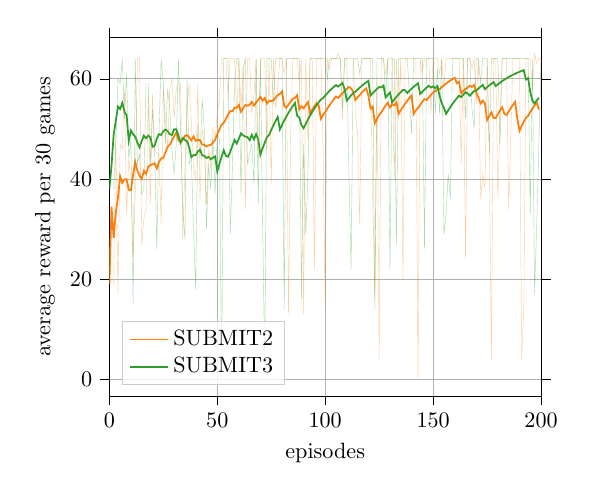
\begin{tikzpicture}[scale=0.8]

\definecolor{color0}{rgb}{1,0.498039215686275,0.0549019607843137}
\definecolor{color1}{rgb}{0.172549019607843,0.627450980392157,0.172549019607843}

\begin{axis}[
legend cell align={left},
legend style={fill opacity=0.8, draw opacity=1, text opacity=1, at={(0.03,0.03)}, anchor=south west, draw=white!80.0!black},
tick align=outside,
tick pos=both,
x grid style={white!69.01960784313725!black},
xlabel={episodes},
xmajorgrids,
xmin=0, xmax=200,
xtick style={color=black},
y grid style={white!69.01960784313725!black},
ylabel={average reward per 30 games},
ymajorgrids,
ymin=-3.25, ymax=68.25,
ytick style={color=black}
]
\addplot [thick, color0]
table {%
0 19
1 34.5
2 28.2736023694928
3 33.4334073251942
4 36.2926114085707
5 40.5393200418368
6 39.2353455238357
7 39.9788027659148
8 39.9818329719994
9 37.8633505238259
10 37.7561990592734
11 40.8301558781599
12 43.4084041178691
13 41.664105307542
14 40.6779702593457
15 40.0211890763431
16 41.6364123355298
17 41.023833557453
18 42.4586519968915
19 42.7688540345797
20 42.9598812251279
21 43.1309431707857
22 42.1330673762052
23 43.4155070655249
24 44.0982120005227
25 44.247219973318
26 45.3100662476348
27 46.4310275365042
28 46.8510326801519
29 47.682805726561
30 48.5186958968966
31 49.2856803041416
32 47.7414437789445
33 47.3282316337224
34 47.8048466471733
35 48.5991039396815
36 48.7683508603447
37 48.2940628075116
38 47.7160740338075
39 48.4983723492815
40 47.6360281873354
41 47.7984064911919
42 47.7437928184608
43 46.8754502256806
44 46.8160136830827
45 46.4901425402958
46 46.7268885565884
47 46.8125107930293
48 47.2275097895103
49 47.814387316336
50 48.894626093678
51 49.9005313155214
52 50.8375052100295
53 51.1799127645466
54 52.0286815348316
55 52.8199193646589
56 53.557696301157
57 53.5209479254647
58 54.2104963227345
59 54.1966629225859
60 54.7745062453744
61 53.4124154997555
62 54.1058680139731
63 54.7532667718175
64 54.638651014225
65 54.7928866277194
66 55.3937841573329
67 54.6507307508485
68 55.2600234902028
69 55.8292363212819
70 56.3610526052909
71 55.6220101472533
72 56.1667117141296
73 55.0511619058371
74 55.6324155041324
75 55.5264315693724
76 55.686961454263
77 56.2262558459517
78 56.7303843521121
79 57.0071771290153
80 57.4603697805553
81 54.5798122617932
82 54.2183987083294
83 54.851807161324
84 55.4440576705631
85 55.9978423433749
86 56.192116847847
87 56.6972789070313
88 53.8706264766204
89 54.5257547394144
90 54.1037619474821
91 54.7436138218176
92 55.3420116464446
93 53.1868319039484
94 53.8856939934125
95 54.539313317799
96 55.1506281527009
97 54.6240172555299
98 51.9995513993998
99 52.7747580093434
100 53.3706425788132
101 54.0571702866154
102 54.6993105452487
103 55.2999389840683
104 55.9263190769865
105 56.4476452827088
106 56.1604718507257
107 56.6666247398946
108 57.1400755102318
109 57.5829398623976
110 57.997196264103
111 58.3846948959656
112 58.0371098023011
113 57.4537793527737
114 55.7462867721453
115 56.2790170581069
116 56.7773485842936
117 57.2435042568915
118 57.6795631149457
119 58.0874696688528
120 56.6620256173733
121 54.0379010333921
122 54.4226579338161
123 51.1687497257269
124 51.9967707412903
125 52.7713462642727
126 53.3023385026454
127 53.9926456341699
128 54.6383999084837
129 55.2424778159894
130 54.2589341895922
131 54.887484483151
132 54.701168975158
133 55.3011724467795
134 53.0233972864893
135 53.7316466971033
136 54.3941924201582
137 55.0139843516821
138 55.5937819130819
139 56.1361663596575
140 56.6435522925419
141 52.9888477208605
142 53.6992958956373
143 54.1703408536327
144 54.8045524518501
145 55.3978421726276
146 55.9528507615105
147 55.7623344137382
148 56.2938224078296
149 56.7910176448371
150 57.2561329614453
151 57.4976823318425
152 57.9172022323809
153 57.9225442088918
154 58.314650837556
155 58.6814586776434
156 59.0246001072055
157 59.3456021648371
158 59.64589334886
159 59.9268099774648
160 60.1896021381819
161 59.0805730153524
162 59.3979614341158
163 57.1141813790768
164 57.5584351313229
165 57.9740264284121
166 58.2337704398514
167 58.6057903161841
168 58.3731557193494
169 58.7361822572389
170 57.2693154359831
171 56.2196712352682
172 55.04419710677
173 55.6219961152534
174 55.0657335520284
175 51.7711437828171
176 52.5601081434336
177 53.2981708414463
178 52.1821525219907
179 52.1704006744929
180 52.9336049982655
181 53.6475697880617
182 54.3154718561069
183 53.0047901123623
184 52.7464154244138
185 53.47245611552
186 54.1516551000329
187 54.7870344699514
188 55.3814213378016
189 52.0664805207609
190 49.6105713381739
191 50.538924125262
192 51.4073828656266
193 52.2198117310888
194 52.5927279421387
195 53.3931987916236
196 54.0129936380829
197 54.6573178157423
198 55.2600725434504
199 53.8239365164739
};
\addlegendentry{SUBMIT2}
\addplot [thick, color1]
table {%
0 38
1 42.65
2 48.82302850796
3 51.6271550129486
4 54.4422768065344
5 53.9644838211898
6 55.1813221789255
7 53.4366342920016
8 52.6594516536824
9 47.6674781124783
10 49.6945269087509
11 48.9103917643466
12 48.4752588981097
13 47.2553791157505
14 46.3109509002112
15 47.5589242147487
16 48.6473332795264
17 48.1260521497745
18 48.6535910132505
19 48.3335571232756
20 46.4213932674238
21 46.6376068968428
22 48.0658150394178
23 48.9495669967927
24 48.794522427477
25 49.5157855504285
26 49.8623358923752
27 49.5676082855018
28 48.921449667865
29 48.7780991675082
30 49.902391723797
31 49.9095343489064
32 48.7553272157814
33 47.2615647382888
34 48.1715677780064
35 47.8046629851976
36 47.5364599983842
37 46.3076032742227
38 44.3349298953628
39 44.7970095944849
40 44.7420187083429
41 45.515315537516
42 45.8220829451443
43 44.7439903612891
44 44.6255864196847
45 44.1772721996067
46 44.4351218668666
47 43.9350778481392
48 44.2747855292304
49 44.5240014990455
50 41.5524394159957
51 43.0472795006655
52 44.4396831838209
53 45.7370404730948
54 44.6289452628474
55 44.4551865452456
56 45.4150032283797
57 46.6396275305058
58 47.7819843894278
59 47.0734137953339
60 48.053181819044
61 49.0987428162486
62 48.6992949025723
63 48.4572404274342
64 48.361976707007
65 47.750482925434
66 48.8109993188691
67 47.9103055766382
68 48.9588724463401
69 47.8543834598685
70 44.8698267187811
71 46.114254570286
72 47.2771103067515
73 48.3638190895433
74 48.7948587387752
75 49.7820465566843
76 50.7047646838138
77 51.5672707100702
78 52.3735351201441
79 49.8858364087268
80 50.8005507294255
81 51.6557341889319
82 52.4552924468734
83 53.202871001085
84 53.9018730073493
85 54.5554758178073
86 55.1666463375906
87 52.6326043533961
88 52.2682472313212
89 50.7633480041644
90 50.1319938317498
91 51.0286446290488
92 51.8672041583321
93 52.6514506547667
94 53.3849147827027
95 54.0708960871556
96 54.71247832353
97 55.3125437455944
98 55.8737864255809
99 56.1403321309447
100 56.6480103912083
101 57.1228598457811
102 57.5670079087156
103 57.9824435616879
104 58.3710264329482
105 58.7344952719826
106 58.4288006471777
107 58.7885006947919
108 59.124960820334
109 57.9548460408347
110 55.6337636720613
111 56.1738288272036
112 56.6790125920569
113 57.1515701872488
114 57.3999719473418
115 57.8259662525451
116 58.2244538134234
117 58.5972121624376
118 58.945903789626
119 59.2720836100691
120 59.5772059439063
121 56.635880105592
122 57.1111147437274
123 57.5556728292887
124 57.9715355250085
125 58.3605559230076
126 58.2727597101408
127 58.6423315849867
128 56.2778762677432
129 56.7761633447472
130 57.2422921845711
131 55.290883375671
132 55.8528408502481
133 56.3785331400257
134 56.8703011662803
135 57.3303346692349
136 57.7606819808977
137 57.7116007818109
138 57.1495090732205
139 57.5915151800898
140 58.0049998998128
141 58.3918039293381
142 58.7536491351065
143 59.0921462290109
144 56.9570342545431
145 57.4114459793328
146 57.8365374672096
147 58.2342007648895
148 58.6062057992907
149 58.2444987418355
150 58.4867993982468
151 58.1327983275641
152 58.5113414852006
153 56.6073180126876
154 55.0842158798344
155 54.1755292436056
156 53.0028811978938
157 53.7123915567711
158 54.3761247032681
159 54.9970342994451
160 55.577883411866
161 56.1212568126592
162 56.6295724863904
163 56.3308850795618
164 56.8256749175425
165 57.2885418027704
166 57.0763747270435
167 56.6198282050264
168 57.095974386458
169 57.5414007019868
170 57.6355049316044
171 58.0461217990016
172 58.4302467208583
173 58.7895889217254
174 57.8999304276967
175 58.2934864467033
176 58.6616513622904
177 59.0060633591765
178 59.3282549266228
179 58.5328787757603
180 58.8855982924672
181 59.2155614592871
182 59.5242364592974
183 59.8129967501569
184 60.0831271759134
185 60.3358296844407
186 60.5722286759547
187 60.7933760064167
188 61.0002556680959
189 61.1937881681243
190 61.3748346245318
191 61.5442005979945
192 61.7026396763491
193 59.8508520186132
194 60.1185395873082
195 57.3366924696629
196 55.6375476751138
197 55.0802855085467
198 55.6557519509981
199 56.1940914023996
};
\addlegendentry{SUBMIT3}
\addplot [very thin, color0, opacity=0.4, forget plot]
table {%
2 19
3 49
4 17
5 47
6 46
7 58
8 33
9 44
10 40
11 24
12 37
13 64
14 64
15 27
16 32
17 34
18 57
19 35
20 57
21 46
22 45
23 45
24 31
25 58
26 52
27 46
28 58
29 60
30 52
31 58
32 59
33 59
34 28
35 42
36 54
37 59
38 51
39 42
40 40
41 59
42 36
43 50
44 47
45 35
46 46
47 42
48 50
49 48
50 53
51 56
52 64
53 64
54 64
55 56
56 64
57 64
58 64
59 53
60 64
61 54
62 63
63 34
64 64
65 64
66 53
67 57
68 64
69 44
70 64
71 64
72 64
73 45
74 64
75 39
76 64
77 54
78 58
79 64
80 64
81 61
82 64
83 13
84 49
85 64
86 64
87 64
88 59
89 64
90 13
91 64
92 48
93 64
94 64
95 22
96 64
97 64
98 64
99 47
100 14
101 64
102 62
103 64
104 64
105 64
106 65
107 64
108 52
109 64
110 64
111 64
112 64
113 64
114 53
115 49
116 31
117 64
118 64
119 64
120 64
121 64
122 36
123 16
124 60
125 4
126 64
127 64
128 61
129 64
130 64
131 64
132 40
133 64
134 52
135 64
136 20
137 64
138 64
139 64
140 64
141 64
142 64
143 0
144 64
145 61
146 64
147 64
148 64
149 53
150 64
151 64
152 64
153 61
154 64
155 58
156 64
157 64
158 64
159 64
160 64
161 64
162 64
163 43
164 64
165 24
166 64
167 64
168 62
169 64
170 55
171 64
172 36
173 41
174 38
175 64
176 47
177 4
178 64
179 64
180 36
181 52
182 64
183 64
184 64
185 34
186 49
187 64
188 64
189 64
190 64
191 4
192 14
193 64
194 64
195 64
196 58
197 65
198 63
199 64
200 64
201 33
};
\addplot [very thin, color1, opacity=0.4, forget plot]
table {%
2 38
3 47
4 60
5 59
6 64
7 52
8 61
9 44
10 48
11 15
12 64
13 43
14 45
15 37
16 38
17 59
18 59
19 43
20 54
21 45
22 26
23 49
24 64
25 59
26 47
27 58
28 54
29 46
30 41
31 47
32 64
33 50
34 34
35 28
36 60
37 43
38 44
39 30
40 18
41 51
42 44
43 56
44 50
45 30
46 43
47 38
48 48
49 37
50 49
51 48
52 0
53 64
54 64
55 64
56 29
57 42
58 59
59 64
60 64
61 37
62 62
63 64
64 43
65 45
66 47
67 39
68 64
69 35
70 64
71 32
72 2
73 64
74 64
75 64
76 55
77 64
78 64
79 64
80 64
81 14
82 64
83 64
84 64
85 64
86 64
87 64
88 64
89 16
90 47
91 29
92 41
93 64
94 64
95 64
96 64
97 64
98 64
99 64
100 64
101 60
102 64
103 64
104 64
105 64
106 64
107 64
108 54
109 64
110 64
111 41
112 22
113 64
114 64
115 64
116 61
117 64
118 64
119 64
120 64
121 64
122 64
123 14
124 64
125 64
126 64
127 64
128 57
129 64
130 22
131 64
132 64
133 27
134 64
135 64
136 64
137 64
138 64
139 57
140 49
141 64
142 64
143 64
144 64
145 64
146 26
147 64
148 64
149 64
150 64
151 53
152 62
153 53
154 64
155 29
156 33
157 41
158 36
159 64
160 64
161 64
162 64
163 64
164 64
165 52
166 64
167 64
168 54
169 50
170 64
171 64
172 59
173 64
174 64
175 64
176 45
177 64
178 64
179 64
180 64
181 47
182 64
183 64
184 64
185 64
186 64
187 64
188 64
189 64
190 64
191 64
192 64
193 64
194 64
195 33
196 64
197 17
198 31
199 47
200 64
201 64
};
\end{axis}

\end{tikzpicture}

        % This file was created by tikzplotlib v0.8.7.
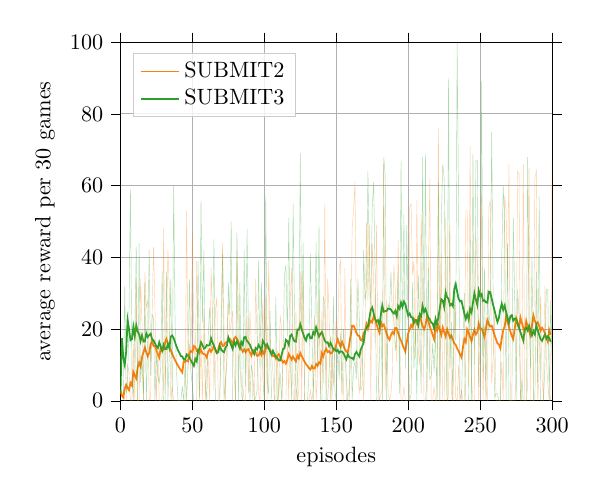
\begin{tikzpicture}[scale=0.8]

\definecolor{color0}{rgb}{1,0.498039215686275,0.0549019607843137}
\definecolor{color1}{rgb}{0.172549019607843,0.627450980392157,0.172549019607843}

\begin{axis}[
legend cell align={left},
legend style={fill opacity=0.8, draw opacity=1, text opacity=1, at={(0.03,0.97)}, anchor=north west, draw=white!80.0!black},
tick align=outside,
tick pos=both,
x grid style={white!69.01960784313725!black},
xlabel={episodes},
xmajorgrids,
xmin=0, xmax=300,
xtick style={color=black},
y grid style={white!69.01960784313725!black},
ylabel={average reward per 30 games},
ymajorgrids,
ymin=0, ymax=100,
ytick style={color=black}
]
\addplot [thick, color0]
table {%
0 3
1 1.45
2 0.934098482043688
3 3.43208472068073
4 4.47139604055284
5 3.59663784068053
6 2.97457589494792
7 5.00700992148582
8 4.29124333284556
9 8.09675157553634
10 7.09185406810066
11 6.26117968444631
12 9.34784545026273
13 10.6928353694924
14 9.60172766868751
15 12.198008852588
16 13.5110158249035
17 14.8484318522405
18 13.5148951809147
19 12.4186612092277
20 13.3246187094393
21 15.8128701407899
22 16.6508503505426
23 15.305050764904
24 15.2807907807425
25 14.0835176579896
26 12.9951112235794
27 12.0797867868609
28 14.7888456678904
29 13.8347288590359
30 14.1423765956914
31 16.1808980014086
32 17.2559962951846
33 16.0140809300585
34 15.1558240137928
35 14.0805708781235
36 13.0879859421535
37 12.1708533206194
38 11.3227024506565
39 10.5377158174314
40 9.81065012747925
41 9.13676868824392
42 8.51178316963302
43 7.9318032553335
44 10.9915977668278
45 10.8568381330402
46 11.2037533844799
47 11.0555414629551
48 13.4663600879188
49 13.903459057626
50 13.5761988716398
51 15.2692343749464
52 14.9855243112285
53 13.9915946432447
54 14.3231819388433
55 13.3764989626543
56 14.2095276524272
57 13.2732168691255
58 12.992028282378
59 12.9268341544685
60 12.0783281009951
61 13.7123298076081
62 14.3861389054426
63 13.6411142590727
64 14.3836751263232
65 15.3383657914916
66 14.3373152189893
67 13.4022974262875
68 14.0929506805603
69 16.0407220725382
70 16.3635101083274
71 15.2990551539555
72 15.4096434142775
73 16.2278065027842
74 16.4078686995155
75 16.7709356254417
76 17.3049862465802
77 16.7013409164266
78 15.6182563846712
79 17.3285452436808
80 17.8257188438603
81 17.3186957721526
82 16.4560220941371
83 15.6494312865734
84 14.6362930840652
85 13.6889567808681
86 14.3562011567813
87 13.5567675717214
88 14.2969976630268
89 14.4071411936193
90 13.4754926749679
91 12.6042202581247
92 13.9873937566456
93 14.1821242971014
94 13.3947856776738
95 12.5291710957895
96 12.624210658873
97 13.6176381675196
98 12.7378870048764
99 13.788389190673
100 12.8977579893574
101 14.5836465775373
102 14.8042857852399
103 14.6877669658937
104 14.2559053428966
105 13.3353862993009
106 12.474353459007
107 12.5728556124364
108 11.7611382293877
109 12.5512570706917
110 13.0321142509201
111 12.1908529562504
112 11.4039265196528
113 10.6678219764289
114 11.0765403999963
115 10.3616126611889
116 11.4354957429462
117 13.0854492005732
118 12.3054639274606
119 11.5112974044552
120 12.381808656548
121 11.5827484032409
122 11.0288710370239
123 12.6403243960383
124 11.8246241314706
125 13.3201449198163
126 12.4606004799145
127 11.6565330324177
128 10.9043606046015
129 10.200732670026
130 9.73609464932533
131 9.10786512402925
132 8.71375391755299
133 9.70009302760093
134 9.07420359052673
135 9.00489215786154
136 10.2950379867056
137 9.75982035163305
138 10.7431503770011
139 10.3725918920056
140 13.2520168812272
141 12.3969821116971
142 13.7908257566981
143 14.5140470974238
144 13.5775978402121
145 13.8629309606293
146 13.2265776752606
147 13.4055173965046
148 14.0245462050763
149 14.2165196493784
150 15.6864838072359
151 17.1906411664886
152 16.0815264722505
153 15.0439726933971
154 16.460536489492
155 15.3985341983617
156 14.4050522043842
157 13.7337407039342
158 13.5573659586139
159 15.779522972761
160 18.1808962273342
161 20.9434751814955
162 20.9471220132956
163 20.1118089662673
164 18.9432857250685
165 18.2372563049483
166 18.092915087369
167 16.9256143472426
168 16.7368626300088
169 18.8828970671611
170 19.4711038138719
171 21.3762137588626
172 19.9970897387678
173 21.5456787279402
174 22.2846735066001
175 21.8792074612218
176 23.6289490858477
177 22.8141724819923
178 21.342280761966
179 20.0943840472305
180 18.9915142493546
181 22.0243360167266
182 20.7969533530787
183 21.2616682170174
184 20.0189744989177
185 18.7274224620703
186 17.6482297772025
187 17.0257611066862
188 18.3789423511702
189 19.193206691568
190 18.6646111588741
191 20.363673171987
192 20.2111777366533
193 18.9072276504221
194 17.6874037677337
195 16.8043436018805
196 15.7201902675223
197 14.7059825760769
198 13.7572078721425
199 16.3535212259345
200 18.8468461961964
201 19.8889866210853
202 21.1219568529322
203 20.5334427812034
204 22.8216104050451
205 22.2524736351355
206 21.4619906663831
207 23.4321866792863
208 23.7914007595572
209 22.2564704085621
210 20.820567980699
211 19.9289177880649
212 21.0302786766392
213 23.6734881785126
214 22.1461654553614
215 20.7173797951212
216 19.6388386037878
217 18.3718161436321
218 17.1865371447663
219 20.9809557143042
220 19.6273451305487
221 21.0062266022414
222 19.6509857051912
223 18.383179763551
224 20.4874913866929
225 19.165717372691
226 17.9937352947056
227 19.9941399674309
228 18.8332274410014
229 17.6181802445086
230 18.2234590618188
231 17.1122679426655
232 16.0082504590561
233 15.6206213324805
234 14.6128391536687
235 13.8636236149602
236 12.9691961627408
237 12.1324737227007
238 14.7690886365357
239 17.2355993230099
240 16.3816895999036
241 19.9054519061788
242 19.008325894585
243 17.7819821834148
244 16.6347574344721
245 18.5292893549405
246 19.7854643233753
247 18.5089826703689
248 19.0567902736479
249 21.5047394288167
250 20.1173368104949
251 20.1742828255826
252 19.0662645266835
253 17.8361828902221
254 20.1693324771598
255 22.4809885353399
256 21.3531827827789
257 20.7497516151795
258 20.9594450659682
259 19.6072227637923
260 18.3422406151206
261 17.1588702223314
262 16.0518463103078
263 15.7259207345438
264 14.7113451818587
265 17.4396455466016
266 19.7338620053461
267 20.6542580209125
268 23.5797898088107
269 22.0585130239369
270 20.6353831312838
271 19.3040680729297
272 18.058644310864
273 17.2161511197565
274 20.234463983455
275 22.9935308512079
276 21.6391094931214
277 20.2430379005321
278 23.1950999959705
279 21.6986419200937
280 20.2987295279826
281 19.2471985835474
282 22.1989922420841
283 20.7667991856902
284 19.4270056823853
285 18.173650470547
286 21.0011569055685
287 23.7752758275218
288 22.2413870579203
289 21.3871040185203
290 21.878258599802
291 20.9183709448536
292 19.5687986214269
293 20.3708116160412
294 19.7662431229572
295 18.8135822737699
296 17.599802769203
297 16.4643316201482
298 19.7246973292046
299 18.4521362085879
};
\addlegendentry{SUBMIT2}
\addplot [thick, color1]
table {%
0 2
1 17.5
2 11.9851906701222
3 10.0605160932297
4 13.68713459297
5 22.5518829210132
6 20.035039967983
7 16.9088540852384
8 17.2077894580914
9 20.6266929986527
10 18.0666894975432
11 21.1042783298687
12 19.3122581920797
13 18.5349270650776
14 16.6436044218558
15 18.252262804609
16 16.5158938947158
17 16.5605796543463
18 18.8452922937542
19 17.8077117443959
20 18.3378856760282
21 18.7287993605453
22 17.1881923953383
23 16.8496831017251
24 16.0663605091108
25 15.1992943870519
26 14.7201987474875
27 16.3440204638421
28 15.1113742786267
29 13.9839843187705
30 15.6100915193055
31 14.4678007630026
32 14.4338626875255
33 15.8420390772776
34 14.710322079117
35 17.9234676100736
36 18.2108355496449
37 17.4953174846737
38 16.2761204116334
39 15.1477204541521
40 14.1025805002939
41 13.4086467243396
42 12.4914504689868
43 12.3898253103161
44 11.5486485555047
45 11.443860673292
46 12.9653116694784
47 12.6313730406438
48 12.0524611378828
49 11.2461543293206
50 10.4955783554641
51 9.79665112999441
52 11.7373466367358
53 11.0251815395372
54 14.0027916491559
55 14.5313628168689
56 16.3440265759018
57 15.5965327345239
58 14.5702410362327
59 14.7956379816168
60 15.5310824751643
61 15.4306962977231
62 15.533480610603
63 17.4615515194642
64 16.3200430004452
65 15.2540710244301
66 14.2585219066442
67 13.3286426735585
68 13.5679053691728
69 15.354489146571
70 14.3551006338357
71 13.8115969353574
72 13.5637829776562
73 14.8268127607777
74 15.4226385020113
75 17.6675601018719
76 16.5209690658877
77 15.4491989888605
78 14.4473160540364
79 16.5576577166433
80 15.4845848042672
81 16.6193967994291
82 15.6724745914978
83 14.6576021192318
84 16.4277385116612
85 15.6233512401631
86 17.7184968366664
87 17.8014087814567
88 16.6498863833711
89 16.2197977402718
90 15.6235926506185
91 14.6134325283275
92 13.7333646212798
93 13.0395753488778
94 14.7174144848183
95 14.347936579921
96 15.5531644299963
97 14.9359358683381
98 13.9710176656592
99 16.750609715498
100 16.056197314355
101 15.1483372678573
102 15.7845896665352
103 14.7652379835289
104 13.8117747914014
105 12.9199337321681
106 13.9581837550738
107 13.0569847414783
108 12.3431336486618
109 12.0627487737914
110 11.2840322284336
111 11.2656971129167
112 12.7977597555463
113 14.4245225649516
114 14.6553062692812
115 17.0011497157205
116 16.6783630201301
117 15.60192819253
118 18.1446483917432
119 18.5225394046392
120 17.3271628400765
121 16.5961641742672
122 16.4931576351778
123 19.8815638071808
124 19.8246750907032
125 21.3847231853691
126 20.0047742416096
127 18.7138904043396
128 17.5063210232748
129 16.8283774711811
130 18.3880874845335
131 18.6211491141428
132 17.4196157805927
133 17.4570648476409
134 19.1697229317991
135 18.5135362718146
136 20.4806166359541
137 19.1591534650452
138 17.9229626000095
139 18.6376731556685
140 19.1772225918656
141 17.9398870039302
142 16.78239143448
143 16.2157472936935
144 16.3308676395407
145 15.2772010451543
146 16.1625918315472
147 15.3133484645435
148 14.3253427276008
149 14.3688709721082
150 13.8289209652868
151 14.1625521739397
152 13.3778423306646
153 13.8050931097394
154 13.7531499355114
155 13.2529315495405
156 12.3978794587196
157 11.59799504696
158 13.0433215596648
159 12.2017974051312
160 11.9952253440151
161 11.9310159526971
162 11.5483624890393
163 12.9968809876521
164 13.6422542395551
165 12.9556465078102
166 12.3778544514024
167 14.2889866407724
168 15.173579416648
169 16.1946509773653
170 19.2789014274394
171 20.4867268350308
172 20.8424253481972
173 22.9816432369703
174 25.434461389508
175 26.0515978419006
176 24.3708370357106
177 22.7985139787334
178 22.1018311020508
179 22.4823604554029
180 21.0318772872047
181 24.0620949736787
182 26.5742304587782
183 24.8597559458019
184 24.9978368124946
185 25.0624927670814
186 25.7681411013194
187 25.6540670726075
188 25.4828363641883
189 24.7420058856231
190 24.3715528049061
191 25.1217772659863
192 23.6300458660397
193 26.4281141513067
194 25.6908148055963
195 27.3881851641738
196 26.2018483020602
197 27.6726995073767
198 26.9841370626092
199 25.2432221883724
200 23.7436572057406
201 24.3408414540733
202 23.3511084415254
203 23.1994238387252
204 21.7026850886945
205 22.5605772999355
206 22.4598947917534
207 21.1399003316444
208 24.1631352416848
209 23.5719647370609
210 26.5028079898173
211 24.7929481720106
212 25.5805004361985
213 24.3172415432246
214 23.1999994911949
215 22.7354831374499
216 21.7848063129289
217 21.605141302342
218 20.2112605856514
219 22.8427932781373
220 21.3690640941637
221 23.2807380887628
222 26.0368204604406
223 28.357026346524
224 27.9468954897257
225 26.143869461154
226 30.26362091526
227 28.8917740629469
228 28.4471433746518
229 26.6118434020963
230 27.0239826214742
231 26.3772739419023
232 31.1271280834719
233 32.5382813458872
234 30.439037060299
235 28.475227930841
236 27.7348905438145
237 27.8810266564429
238 26.0822505280174
239 24.3995244992538
240 22.8253614635943
241 24.2559834447115
242 22.6910811436674
243 25.6787535839182
244 24.6672210135605
245 27.3983682497182
246 29.9533124128117
247 28.2789050505059
248 26.7125239833582
249 30.7310710538934
250 29.2645502619617
251 29.7636115604621
252 27.8433784662923
253 28.0470314774229
254 27.4633520032544
255 27.3689421929595
256 30.4419137750154
257 30.3488870767201
258 28.455410431468
259 26.7486097081639
260 25.1519251668385
261 23.5292202755096
262 22.0112060275575
263 23.107257276327
264 25.4874342765022
265 27.0688901608713
266 25.3225101182201
267 26.527509486263
268 24.816057233665
269 23.2150212588844
270 21.7172779306625
271 23.606485831116
272 23.8899383616514
273 22.3486519978805
274 22.906803487938
275 22.9773322958829
276 21.4949237466034
277 20.495251237952
278 19.1729769535596
279 17.9360106888857
280 16.7788487005514
281 20.0834391294247
282 20.3361204775198
283 19.6047578617173
284 20.9205799424755
285 19.5708651004524
286 18.3082286362112
287 19.4496332455253
288 18.5173988386161
289 21.0001473105369
290 19.645299091902
291 18.3778604363905
292 17.1921920172705
293 16.728179627643
294 17.6489422349406
295 18.5103008027294
296 17.3160878447301
297 18.0053725015203
298 17.5534129843047
299 16.4209347249358
};
\addlegendentry{SUBMIT3}
\addplot [very thin, color0, opacity=0.4, forget plot]
table {%
2 3
3 0
4 0
5 10
6 8
7 0
8 0
9 16
10 0
11 33
12 0
13 0
14 34
15 22
16 0
17 36
18 26
19 28
20 0
21 1
22 23
23 43
24 26
25 0
26 15
27 0
28 0
29 1
30 48
31 2
32 18
33 42
34 31
35 0
36 4
37 0
38 0
39 0
40 0
41 0
42 0
43 0
44 0
45 0
46 53
47 9
48 16
49 9
50 47
51 20
52 9
53 39
54 11
55 0
56 19
57 0
58 26
59 0
60 9
61 12
62 0
63 37
64 24
65 3
66 25
67 29
68 0
69 0
70 24
71 44
72 21
73 0
74 17
75 28
76 19
77 22
78 25
79 8
80 0
81 42
82 25
83 10
84 4
85 4
86 0
87 0
88 24
89 2
90 25
91 16
92 0
93 0
94 34
95 17
96 2
97 0
98 14
99 28
100 0
101 29
102 0
103 39
104 18
105 13
106 8
107 0
108 0
109 14
110 0
111 24
112 20
113 0
114 0
115 0
116 17
117 0
118 27
119 37
120 1
121 0
122 25
123 0
124 3
125 36
126 0
127 35
128 0
129 0
130 0
131 0
132 3
133 0
134 3
135 24
136 0
137 8
138 29
139 2
140 25
141 5
142 55
143 0
144 34
145 25
146 0
147 18
148 4
149 16
150 23
151 17
152 37
153 39
154 0
155 0
156 37
157 0
158 0
159 4
160 11
161 48
162 53
163 61
164 21
165 8
166 2
167 8
168 16
169 0
170 14
171 50
172 28
173 49
174 0
175 44
176 33
177 16
178 49
179 11
180 0
181 2
182 3
183 66
184 3
185 28
186 2
187 0
188 2
189 8
190 38
191 31
192 11
193 45
194 18
195 0
196 0
197 4
198 0
199 0
200 0
201 54
202 55
203 35
204 39
205 12
206 56
207 14
208 10
209 52
210 29
211 0
212 0
213 7
214 37
215 62
216 0
217 0
218 4
219 0
220 0
221 76
222 0
223 41
224 0
225 0
226 51
227 0
228 1
229 49
230 2
231 0
232 27
233 1
234 0
235 10
236 0
237 3
238 0
239 0
240 53
241 53
242 4
243 71
244 6
245 0
246 0
247 46
248 38
249 0
250 27
251 57
252 0
253 21
254 3
255 0
256 54
257 56
258 5
259 12
260 24
261 0
262 0
263 0
264 0
265 11
266 0
267 57
268 53
269 34
270 66
271 0
272 0
273 0
274 0
275 5
276 64
277 63
278 2
279 0
280 66
281 0
282 0
283 4
284 65
285 0
286 0
287 0
288 62
289 64
290 0
291 9
292 29
293 7
294 0
295 32
296 11
297 5
298 0
299 0
300 67
301 0
};
\addplot [very thin, color1, opacity=0.4, forget plot]
table {%
2 2
3 32
4 2
5 5
6 26
7 59
8 8
9 0
10 19
11 43
12 0
13 44
14 5
15 12
16 0
17 33
18 0
19 17
20 42
21 7
22 24
23 23
24 0
25 13
26 7
27 5
28 9
29 36
30 0
31 0
32 36
33 0
34 14
35 34
36 0
37 60
38 22
39 8
40 0
41 0
42 0
43 4
44 0
45 11
46 0
47 10
48 34
49 8
50 4
51 0
52 0
53 0
54 39
55 1
56 56
57 22
58 42
59 5
60 0
61 18
62 26
63 14
64 17
65 45
66 0
67 0
68 0
69 0
70 17
71 41
72 0
73 6
74 10
75 33
76 24
77 50
78 0
79 0
80 0
81 47
82 0
83 33
84 2
85 0
86 42
87 4
88 48
89 19
90 0
91 10
92 7
93 0
94 1
95 3
96 39
97 9
98 33
99 6
100 0
101 57
102 6
103 2
104 25
105 0
106 0
107 0
108 29
109 0
110 2
111 8
112 0
113 11
114 35
115 38
116 18
117 51
118 12
119 0
120 55
121 24
122 0
123 6
124 15
125 69
126 19
127 44
128 0
129 0
130 0
131 7
132 41
133 22
134 0
135 18
136 44
137 9
138 49
139 0
140 0
141 29
142 27
143 0
144 0
145 8
146 18
147 0
148 29
149 3
150 0
151 15
152 6
153 19
154 2
155 20
156 13
157 6
158 0
159 0
160 34
161 0
162 9
163 11
164 6
165 34
166 23
167 3
168 4
169 42
170 28
171 31
172 64
173 38
174 26
175 54
176 61
177 35
178 0
179 0
180 12
181 28
182 0
183 68
184 63
185 0
186 27
187 26
188 36
189 24
190 23
191 14
192 19
193 36
194 2
195 67
196 15
197 52
198 9
199 49
200 17
201 0
202 2
203 33
204 9
205 21
206 0
207 35
208 21
209 2
210 68
211 15
212 69
213 0
214 37
215 6
216 7
217 16
218 8
219 19
220 0
221 61
222 0
223 51
224 66
225 62
226 22
227 0
228 90
229 9
230 22
231 0
232 33
233 17
234 100
235 53
236 0
237 0
238 17
239 30
240 0
241 0
242 0
243 45
244 0
245 69
246 10
247 67
248 67
249 4
250 4
251 89
252 8
253 37
254 0
255 31
256 19
257 26
258 75
259 29
260 1
261 2
262 2
263 0
264 0
265 39
266 60
267 50
268 0
269 44
270 0
271 0
272 0
273 51
274 28
275 0
276 31
277 24
278 0
279 6
280 0
281 0
282 0
283 68
284 24
285 9
286 40
287 0
288 0
289 36
290 5
291 57
292 0
293 0
294 0
295 10
296 31
297 31
298 0
299 28
300 11
301 0
};
\end{axis}

\end{tikzpicture}

        \caption{Log agent results for the \texttt{Treechop} (left) and \texttt{ObtainDiamondDense} environments (right).}
        \label{fig:submits}
    \end{figure}

    \begin{table}[ht]
        \caption{Comparison of the algorithms implemented for the \texttt{Treechop} environment.}
        \centering
        \label{tab:algos}
        \begin{tabular}{llllll}

            \toprule
            & Demonstrations & Discretization & Embeddings & Episodes & Reward \\
            \midrule
            SAC            &                &                &            & 300      & 5      \\
            GAIL           & +              & +              & +          & 150      & 30     \\
            RnD            &                & +              & +          & 1000     & 35     \\
            PPO            &                & +              & +          & 1000     & 35     \\
            Pretrained PPO & +              & +              & +          & 150      & 50     \\
            \textbf{HDQfD} & +              & +              &            & 200      & 60     \\
            \bottomrule
        \end{tabular}

    \end{table}


    \section{Conclusion}\label{sec:conclusion}
    In this paper we introduce a novel approach to learn from imperfect demonstrations.
    This hierarchical Deep Q-Network from Demonstrations won first place in the MineRL competition and received \textbf{61.61} score.
    In our further work, we plan to train all item agents for full hierarchical end-to-end architecture.
    Besides, for these agents we plan to ensure access to all demonstrations from all substasks with respect to the agent's inventory for additional performance.

    \subsubsection*{Acknowledgments}

    This work was supported by the Russian Science Foundation, project no.
    18-71-00143.
    We thank the AIM Tech Company for its organizational and computing support.

    \medskip

    \small
    \bibliographystyle{abbrvnat}
    \bibliography{nips}


\end{document}